% !TEX root =../dissertation.tex
\documentclass[./dissertation.tex]{subfiles}
\begin{document}
\chapter{Minimally-Supervised Biomedical image Segmentation via Contrastive Learning}
\label{ch:contrastive}
% \lipsum[7]

\section{Introduction}

\label{biomed/image segmentation}
Image segmentation is a fundamental process in many computer vision applications and is used to partition the image into separate regions. It is an essential part in various biomedical applications, including lesion and tumor detection and analysis, organ localization and identification, diagnosis and monitoring, and cell and tissue analysis. Similarly, image segmentation is a cornerstone of quantitative cell research, particularly for studying cellular dynamics like motility \cite{vaezi2022novel} and morphological changes. Given its critical role, it has been the focus of extensive research, with ongoing advancements aimed at improving accuracy, automation, and generalization across diverse imaging modalities.

\label{biomedical images nature}
Biomedical images come in a vast variety of formats, types, and modalities \cite{liu2022multi,vicar2019cell,zhou2019review}. Similarly, due to the variety of biological structures, segmentation targets can vary from nuclei and cell membranes to organelles such as mitochondria, cilia, tumors, and lesions, as well as blood vessels, bone, and brain structures \cite{vaezi2024training}. \label{CNNs} Deep learning (DL) has advanced the field of image segmentation, particularly with the success of convolutional neural networks (CNN) \cite{weng2021inet}. While CNNs revolutionized segmentation for their high accuracy, due to the large diversity in biomedical image modalities, formats, and structures as well as the scarcity of ground truth data, CNNs are tailored for specific tasks \cite{ma2023towards} in biomedical image segmentation and therefore suffer from overfitting and exhibit poor generalizability over unseen data. Furthermore, their specificity to tasks, high computational demands, and complex implementation limit their broader application.

\label{SAM}
Inspired by Large Language Models (LLMs), Foundation Models such as the Segment Anything Model (SAM) \cite{kirillov2023segment} demonstrate excellent zero-shot segmentation performance across a large variety of general images. Studies that build upon SAM \cite{kim2024medivistamedicalvideosegmentation} have shown promising zero-shot learning capabilities and can segment objects in biomedical images regardless of their modality. However, when applied to biomedical data without fine-tuning, SAM often struggles to match the accuracy of domain-specific models like U-Net. Its zero-shot performance varies significantly across medical datasets and tasks, highlighting the need for fine-tuning to adapt it effectively for biomedical image segmentation. Furthermore, although SAM excels at segmenting objects with well-defined, envelope or convex geometries, it struggles with biological structures that exhibit diffuse or punctate patterns such as cilia, which are even difficult to generate hand-drawn labels for.

\label{Unsupervised}
Unsupervised methods, on the other hand, are used in scenarios where domain-specific cues suffice for crafting an algorithm for segmentation and when obtaining ground truth data is costly \cite{vaezi2024training}. However, since they are domain-specific, unsupervised methods also exhibit poor generalizability. Self-supervised learning (SSL) is also a promising direction in unsupervised segmentation. Contrastive learning (CL) is a successful variant of SSL and refers to a type of learning where the goal is to learn representations by contrasting positive pairs (similar or related data points) against negative pairs (dissimilar or unrelated data points). This approach is widely used in self-supervised learning where labels are not available. Contrastive coding (CC), often seen as a subset or a specific implementation of CL, refers more specifically to the encoding process where contrastive loss functions are used to train models to produce these discriminative embeddings.

\label{Contrastive}
Contrastive learning provides an alternative approach to segmentation by leveraging similarities and differences in the data rather than relying on explicit labels. For addressing all the aforementioned issues, we turned to contrastive coding to teach the network to recognize objects of the same texture and configuration. By learning representations that cluster visually similar structures together while separating dissimilar ones, contrastive learning enables segmentation with minimal user interaction. This makes it particularly suitable for biomedical image analysis, where labeled data is scarce, and manual annotations are costly and time-consuming. The code to our method is available at \url{https://github.com/quinngroup/contrastive-coding}

\label{PaperStructure}
The rest of this paper is structured as follows. Section~\ref{Methodology} describes our proposed contrastive learning approach for biomedical image segmentation, detailing the network architecture and training procedure, and presents the experimental setup and datasets used to evaluate our method. Section~\ref{Results and Discussion} discusses the segmentation performance and compares it with existing approaches. Finally, Section~\ref{Conclusion} concludes the paper with a summary of findings and potential directions for future research.

% 1- Maybe start with advances in biomedical image segmentation, like CNN and SAM methodologies.  \\
% move to he background section?
% The Segment Anything Model (SAM) [35] can segment an object within an image using user inputs, including a single point, multiple points, an entire mask, a bounding box, or textual descriptions. This functionality is based on the model's inherent ability to recognize objects, which enables it to segment unfamiliar object types without further training, effectively supporting zero-shot learning.

% 2- Continue with mentioning that these methods need either large-scale annotated datasets, or, fine-tuning for domain adaptation like in the case of SAM2 and the adaptations for biomed purposes. Also don't forget to mention that some biomed structures are inherently difficult to even hand-annotate because of their shape (refer to Shannon's email for better wordings.) \\

% 3- Say that quality annotated biomed data in large quantity is scarce and crafting one is expensive, time-consuming, and is different from general images since it needs an expert's opinion. \\

% 4- move on by introducing the unsupervised or semi-supervised methods and mention that they're an option when annotated data is unavailable. say that they use domain specific knowledge to invent a way to segment, like what we did with optical flow and cilia structure. \\



% 5- and finalize with contrastive learning and that it can be used with minimal user interaction on unannotated biomed data to generate accurate segmentations. \\

% 6- Then there's the structure of the paper.



\label{Background}
\section{Background}

Image segmentation is a crucial topic in computer vision and in particular deep learning. In image segmentation, an input image is broken down into its mutually exclusive semantic constituents such as the independent objects and the background. To address the first aforementioned shortcoming, Hyunseob et al. proposed a model called MDNet \cite{nam2016learning}. MDNet, or Multi Domain Network, is a supervised tracking method that learns domain-independent representations from pre-training. In supervised learning, a set including different objects which are semantically similar together, such as "pedestrian", "ball", "car", or "flower," are used for training. The most important drawback of MDNet, and any supervised segmentation framework like Mask- and Cascade-RCNN \cite{he2018maskrcnn,cai2018cascade} SSD \cite{liu2016ssd}, is that it relies on large amounts of labeled data for training from various objects, while after training the model with such a big dataset, there is still no guarantee that it can detect any other objects. There always exists sets of objects which are not used for training, and as a consequence, the network may not detect those types of objects properly.

Some unsupervised segmentation methods were proposed recently \cite{croitoru2019unsupervised,ji2019invariant,liu2014mslrr,xia2017w}, the most popular of which is W-Net \cite{xia2017w}. However, since W-Net has to reconstruct the entire image again from the segmentation map, background and other objects of no interest have to be present in the segmentation mask, increasing the burden on the network to perfectly segment them, while they are of no interest. Indeed, we first started our experimentation to try to extend the work in W-Net, but we found it relied heavily on the final Conditional Random Field (CRF) module to fix the background creeping, and we could not distill the objects of interest alone with the segmentation mask. Also, in \cite{croitoru2019unsupervised}, an unsupervised segmentation method was proposed for separating the background from foreground using deep learning, and again, distilling the object of interest alone is still an issue in this work, since sometimes the object of interest is visually closer to the background than to the foreground, as in some of our data that we present later.

For addressing all the aforementioned issues we turned to contrastive coding in order to teach the network to recognize objects of the same texture and con guration. In contrastive coding, the goal is to represent instances (images/videos/patches) with vectors, and have instances that are similar attract and instances that are dissimilar repel each other. This is typically done with dot product or cosine similarity on the learnt vectors. There has been a lot of recent work in unsuper vised contrastive learning \cite{oord2018representation,he2020momentum,chen2020improved}, such as SimCLR\cite{chen2020simple,chen2020big}, where patches from the same image are made to attract each other, while patches from different images are made to repel each other. To aid with better object recognition, the patches are transformed with the usual image augmentation techniques like color jittering, blurring, flipping, and rotation.


% 1- Again, start with advances in biomed segmentation methods. mention U-Net and its variants, then mention the newly emerged SAM, then mention some of the adaptations of SAM 2 for biomed. End this section by restating the problem with biomed data. You can cite your Toxo paper here. \\

% 2- move on with unsupervised methods and briefly mention the SOTA out there. you can cite your paper on Cilia here and use it as an example of an unsupervised method. Quickly introduce CL and explain how it has been used to segment. You can cite SimCLR and similar ones. \\

% 3- Briefly touch on YOUR method of using CL for biomed segmentation, such as, finding the similar and/or dissimilar samples from consecutive frames, your modified contrastive loss, your modified architecture. should I really talk this much about the method in here? no!


\label{Methodology}
\section{Methodology}
\begin{figure}
    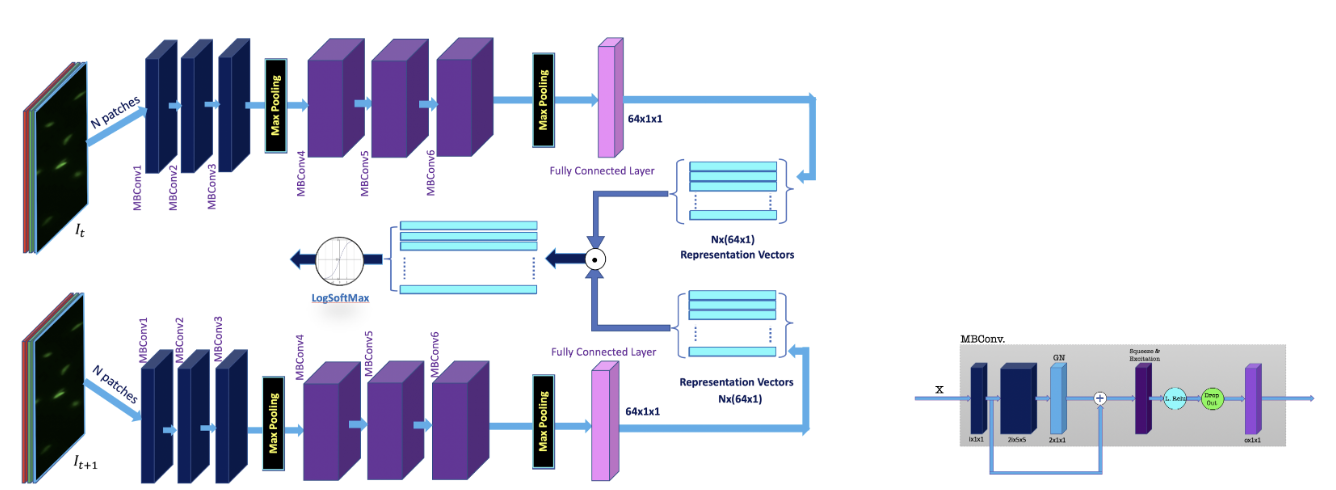
\includegraphics[width=\textwidth]{./figures/cc/arch.png}
    \caption{(a) The architecture of our contrastive network applied to two consecutive frames. (b) The internals of an MBConv layer.} \label{fig:architecture}
\end{figure}

\subsection{Network architecture}
The network is designed to take in a patch of dimensions \(i \times k \times k\) and output a vector of size \(d\) to represent this patch in the dot product operations. We achieve this with a network constructed as follows: Three MBConv layers each outputting 32 channels, followed by a max pooling layer that downsizes the image by half, then another 3 MBConv layers each outputting 64 channels, followed by a global max pooling layer downsizing the image to \( d \times 1 \times 1\) followed by a fully connected layer that outputs another \(d\)-dimensional vector with a final activation function of \(tanh\). Figure~\ref{fig:architecture}(a) illustrates the network architecture and the application of the network to the current and next video frames. An MBConv layer is adapted from EfficientNet\cite{tan2019efficientnet}. Figure~\ref{fig:architecture}(b) shows the internals of an MBConv layer. \\


\subsection{Contrastive training}

Let \(x_1, x_2, \ldots, x_N\) be patches of size \(i \times k \times k\) pixels from an input image \(I_t\). We aim to represent each patch with a vector representation of size \(d\). The vector representation of a patch \(x_i\) is obtained using a convolutional neural network, whose final output layer produces a \(d\)-dimensional vector, i.e., \(v_i = f_\theta(x_i)\), where \(\theta\) represents the parameters of the neural network \(f\).

% 2- then the trick of using consecutive frames for selecting similar and dissimilar patches.
The goal of contrastive learning is to bring similar vectors closer together while pushing dissimilar ones farther apart. To achieve this, we need to sample vectors that should be similar and others that should be dissimilar. We use the observation that our videos are Nyquist sampled, i.e., the sampling rate in our videos is high relative to the frequency of the recorded motion. This implies that consecutive frames differ only slightly in content. Therefore, a patch \(x_i\) from the same location in two consecutive frames \(I_t\) and \(I_{t+1}\) will most likely be similar, and this forms the basis for sampling positive examples.

For negative examples, however, we sample random patches from both the current frame and the next frame. Even though these random patches might contain objects visually similar to the current patch, we assume that the corresponding patch from the next frame will be the most similar to the current patch and should thus be coupled positively above any other pairing. We set a ratio of \(m : 1\) for negative to positive samples to contrast with the vectors from the current frame.


\begin{table}
    \caption{Cell Tracking Challenge (CTC) 2D Datasets}
    \centering

    \label{tab:ctc_datasets}
    \begin{tabular}{|l|l|l|}
        \hline
        \textbf{Dataset Name} & \textbf{Modality}    & \textbf{Cell Type}                  \\ \hline
        BF-C2DL-HSC           & Brightfield (BF)     & Mouse hematopoietic stem cells      \\ \hline
        BF-C2DL-MuSC          & Brightfield (BF)     & Mouse muscle stem cells             \\ \hline
        DIC-C2DH-HeLa         & DIC                  & HeLa cells on a flat glass          \\ \hline
        Fluo-C2DL-Huh7        & Fluorescence (Fluo)  & Human hepatocarcinoma-derived cells \\ \hline
        Fluo-C2DL-MSC         & Fluorescence (Fluo)  & Rat mesenchymal stem cells          \\ \hline
        Fluo-N2DH-GOWT1       & Fluorescence (Fluo)  & GFP-GOWT1 mouse stem cells          \\ \hline
        Fluo-N2DL-HeLa        & Fluorescence (Fluo)  & HeLa cells expressing H2b-GFP       \\ \hline
        PhC-C2DH-U373         & Phase Contrast (PhC) & Glioblastoma-astrocytoma U373 cells \\ \hline
        PhC-C2DL-PSC          & Phase Contrast (PhC) & Pancreatic stem cells               \\ \hline
        Fluo-N2DH-SIM+        & Fluorescence (Fluo)  & Simulated nuclei of HL60 cells      \\ \hline
    \end{tabular}
\end{table}




% 3- then describe the datasets you'll be testing it on.
\subsection{Datasets}


To evaluate the performance of our proposed segmentation method, we utilize a diverse set of biomedical video datasets. By incorporating datasets with a wide range of cell shapes, sizes, and motility patterns, we aim to assess the generalizability of our method across different biological structures and imaging conditions. By applying our method to these datasets, we also aim to evaluate its ability to handle complex, diffuse, or punctate patterns.

\subsubsection{Cell Tracking Challenge Datasets}
We use all available 2D datasets from the Cell Tracking Challenge (CTC)~\cite{mavska2023cell}. These datasets include various cell types and imaging modalities, such as fluorescence and phase-contrast microscopy images. They cover a range of biological structures and provide a diverse testbed for evaluating the performance of segmentation methods across different imaging conditions.

% \subsubsection{Cilia Motion Datasets}
% In addition to the CTC datasets, we include videos of both kinetic and dyskinetic cilia. These datasets capture the motion of cilia under normal and impaired physiological conditions. The kinetic cilia datasets represent coordinated, functional movement, while the dyskinetic cilia datasets exhibit irregular or impaired motion.


% This allows us to assess the model's ability to segment structures with varying motion dynamics and handle complex spatial patterns characteristic of ciliary motion.
\subsection{Training process}

Each iteration of the training, we construct the matrix \(R^{n \times d}\) which is the set of patches of an image \(I_t\) after passing them through the representation network where column \(i\) represents \(v_i = f_\theta(x_i)\). To represent the similarity with all the negative and positive samples, we construct the matrix \(M ^{n \times (m+1)}\) where each column is the dot product between the matrix \(R\) with a matrix \(Q^{n\times d}\) of random patches sampled randomly from the \(2N\) available patches at hand from the current \(I_t\) and next \(I_{t+1}\) frames, except for the last column, the column of positive patches, where the matrix \(Q\) is set to be the vectors of the next patches of the matrix R from the next frame \(I_{t+1}\). We also transform the next-frame positive patches by flipping them horizontally and vertically each with probability \(0.5\). This is so that the network learns to associate the same texture in different positions and configurations.

\subsection{Similarity and loss}
We choose the cosine similarity between vectors as our similarity metric. The vector output of the convolutional network is, therefore, projected onto the \(L2\) unit sphere (i.e., normalized), before being used with dot products. For practical numerical stability, though, we use logSoftmax with negative log-likelihood instead of softmax and cross-entropy.




% 4- use figures, tables, graphs here.

\label{Results and Discussion}
\section{Results and Discussion}

We evaluate our method on a subset of 2D datasets from the CTC. The CTC offers a diverse array of 2D and 3D time-lapse microscopy datasets, each capturing unique biological specimens under various imaging modalities. Table~\ref{tab:ctc_datasets} contains an overview of these datasets, detailing the organisms studied, imaging techniques employed, and acquisition specifics.

For each dataset, or part of dataset, we leave out 20\% of the data as a testing portion, and of the remaining 80\%, we take 70\% of it for training, and 30\% for validation. We use the loss on the validation to choose the best model, and report the dice coefficient using the best trained model on the testing portion. In each iteration we sample 1024 patches within the input image, and construct the matrix with the number of negative samples \(m = 9\), and the size of representation vector \(d = 64\). As noted before, the contrastive loss only minimizes a lower bound on the error, so the training error of the negative log likelihood loss never goes down to \(0\). We train to 50 epochs for each part of the dataset and use the Adam optimizer as well with the same \(10e^-3\) learning rate. To generate masks we take user's input in the form of at least one point indicating the coordinates of the object of interest. These coordinates represent the center of the patch whose representation vector will be the anchor to compare against. We sweep the entire image with patches of size \({15}\times{15}\) and stride of 1, generating a representation vector per each pixel in the image, and report the dot product of these vectors and the anchor vector. We use reflective padding instead of zero padding. Finally, the user can select a suitable threshold to binarize the raw mask into the final mask.

\begin{figure}
    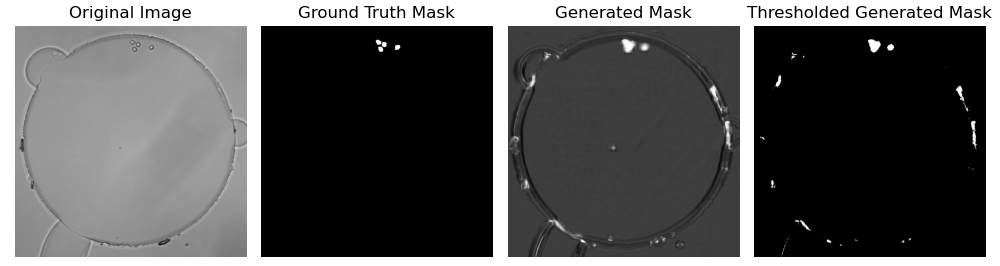
\includegraphics[width=0.5\textwidth]{./figures/cc/BF-C2DL-HSC.png}
    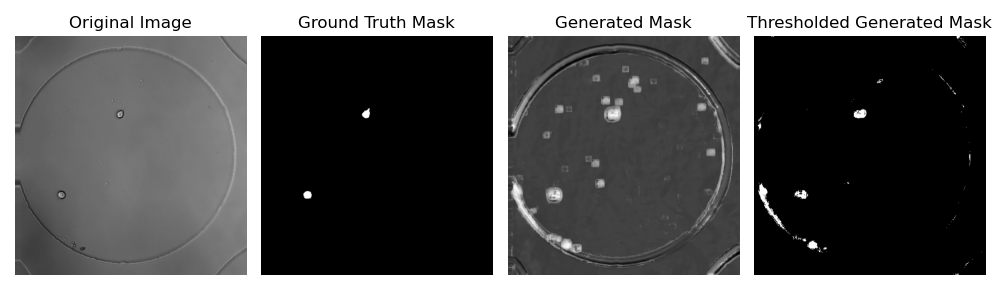
\includegraphics[width=0.5\textwidth]{./figures/cc/BF-C2DL-MuSC.png}
    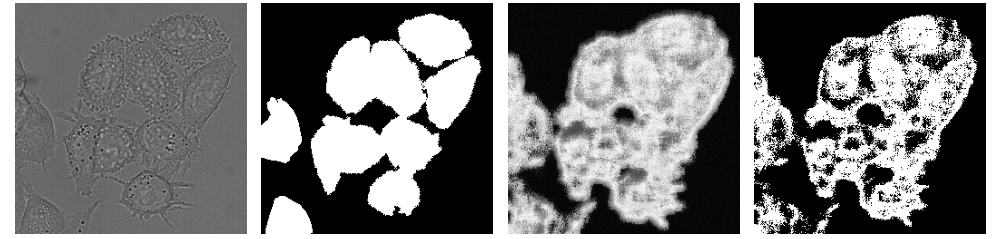
\includegraphics[width=0.5\textwidth]{./figures/cc/DIC-C2DH-HeLa.png}
    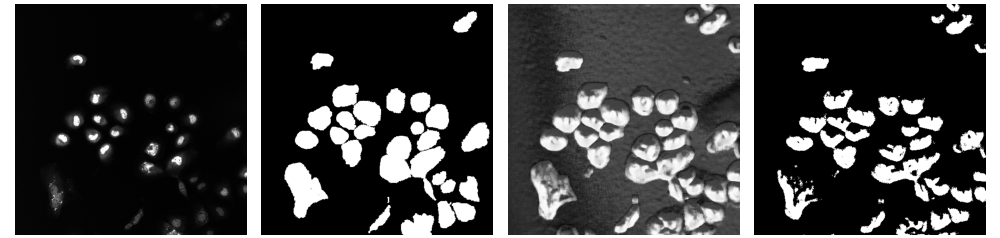
\includegraphics[width=0.5\textwidth]{./figures/cc/Fluo-C2DL-Huh7.png}
    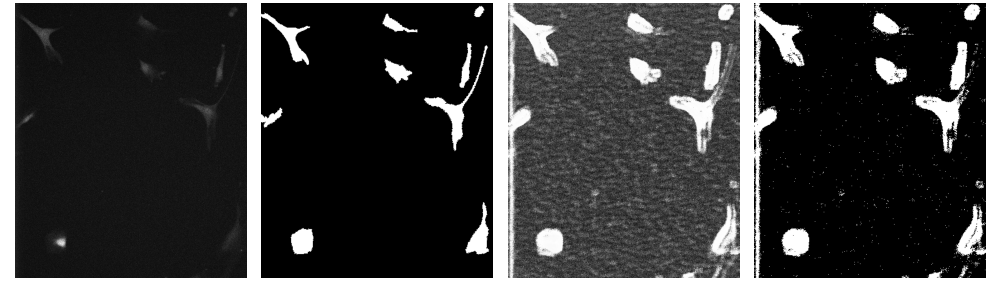
\includegraphics[width=0.5\textwidth]{./figures/cc/Fluo-C2DL-MSC.png}
    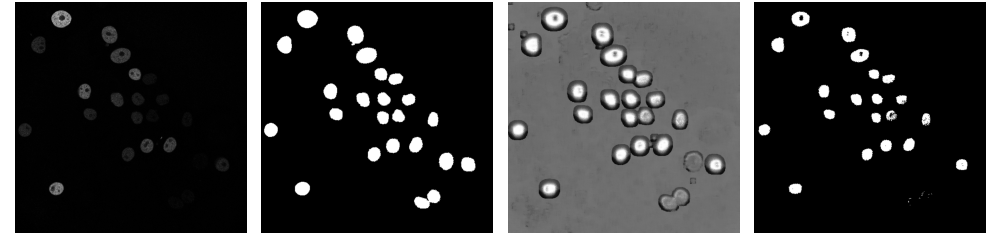
\includegraphics[width=0.5\textwidth]{./figures/cc/Fluo-N2DH-GOWT1.png}
    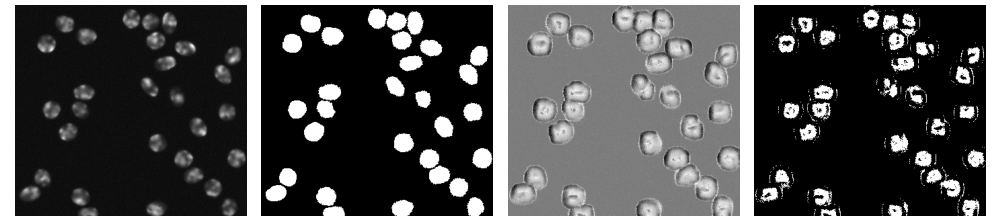
\includegraphics[width=0.5\textwidth]{./figures/cc/Fluo-N2DH-SIM+.png}
    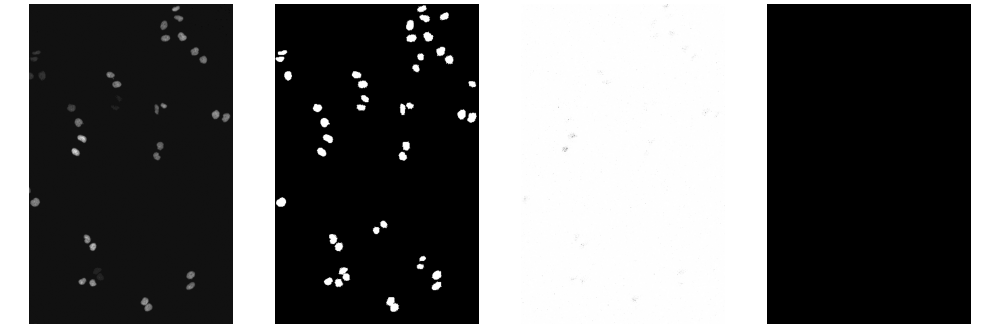
\includegraphics[width=0.5\textwidth]{./figures/cc/Fluo-N2DL-HeLa.png}
    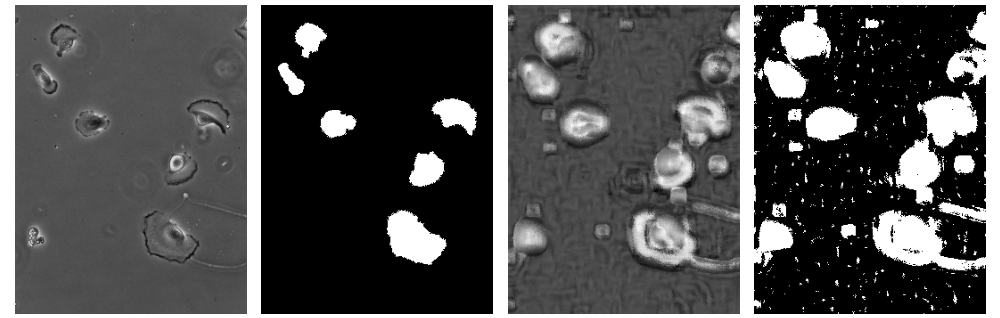
\includegraphics[width=0.5\textwidth]{./figures/cc/PhC-C2DH-U373.png}
    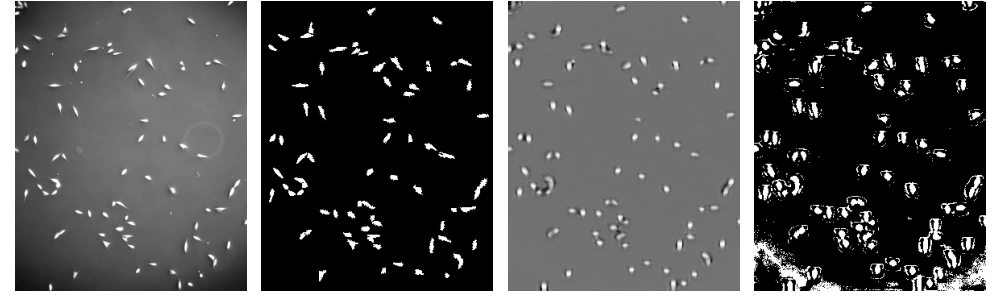
\includegraphics[width=0.5\textwidth]{./figures/cc/PhC-C2DL-PSC.png}
    \caption{Visual comparison of segmentation performance across different datasets. The variation in performance across datasets indicates the challenges caused by different imaging modalities and cell types.} \label{fig2}
\end{figure}


\begin{table}
    \caption{Dice coefficients and intersection-over-union (IoU) scores for the CTC datasets.}
    \centering
    \label{tbl:iou_dice}
    \begin{tabular}{|l|l|l|l|l|l|l|l|l|l|l|}
        \hline
        \textbf{Dataset Name} & \textbf{IoU} & \textbf{Dice} \\ \hline
        Fluo-N2DH-GOWT1       & 0.815        & 0.8971        \\ \hline
        Fluo-N2DL-HeLa        & 0.487        & 0.655         \\ \hline
        PhC-C2DL-PSC          & 0.736        & 0.847         \\ \hline
        Fluo-C2DL-Huh7        & 0.617        & 0.762         \\ \hline
        Fluo-N2DH-SIM+        & 0.786        & 0.7404        \\ \hline
        BF-C2DL-HSC           & 0.206        & 0.341         \\ \hline
        BF-C2DL-MuSC          & 0.15         & 0.261         \\ \hline
        DIC-C2DH-HeLa         & 0.551        & 0.711         \\ \hline
        Fluo-C2DL-MSC         & 0.419        & 0.591         \\ \hline
        PhC-C2DH-U373         & 0.342        & 0.51          \\ \hline
    \end{tabular}
\end{table}

Table~\ref{tbl:iou_dice} shows a mix of strong and moderate results for dice coefficients and precision. The BF-C2DL-HSC and BF-C2DL-MuSC datasets exhibit the weakest performance, with Dice scores of 0.341 and 0.261, respectively. This poor performance is due to the brightfield imaging modality, which introduces significant intensity variations and makes boundary segmentation challenging. Additionally, artifacts and shadows within the hydrogel environment likely contribute to false positives and inconsistent mask predictions. The DIC-C2DH-HeLa dataset achieves a moderate Dice score of 0.711, showing a reasonable ability to capture cell structures. However, the fine-grained details of the HeLa cells in differential interference contrast (DIC) imaging pose difficulties in maintaining sharp boundary delineation, leading to a loss in segmentation accuracy.

For the Fluo-C2DL-MSC dataset, the Dice coefficient of 0.591 indicates moderate segmentation quality. The elongated morphology of mesenchymal stem cells complicates boundary definitions, leading to thresholding artifacts. The PhC-C2DH-U373 dataset, with a Dice coefficient of 0.510, shows lower performance due to halo effects in phase contrast imaging, which interfere with precise boundary extraction and introduce noise.

Overall, the results suggest that datasets with clear and well-defined fluorescence-stained boundaries (such as GOWT1) tend to perform best, while datasets relying on phase contrast, brightfield, or DIC imaging suffer from boundary inconsistencies and intensity variations that complicate segmentation.

% Regarding the cilia dataset, Figure 2(b) illustrates the application of our method, where it is evident that the segmentation does not simply isolate the background, nor does it mistakenly include the cilia as foreground. This suggests that conventional background/foreground segmentation methods would not be effective. Nonetheless, our approach successfully identifies the cell regions where cilia are attached, albeit with minor false positives in the lower-left corner.% 2- use figures, tables, and graphs here.

\label{Conclusion}
\section{Conclusion and Final Remarks}

We have introduced a method for object segmentation using contrastive coding, requiring minimal user input to select the object of interest. By enforcing similarity between temporally adjacent patches and differentiating dissimilar ones, the model learns embeddings that enable segmentation without the need for labeled datasets. Our approach generates visually plausible masks and demonstrates good results in some datasets, although it achieves only moderate performance in others. We discuss the reasons for these varying results and emphasize the novelty of our method. Additionally, we provide a GUI tool to assist users in marking the object of interest and setting the appropriate threshold for the entire video.

While our results are encouraging, there are several avenues for future work. First, refining the segmentation boundaries through post-processing or boundary-focused contrastive objectives could help address residual errors in challenging datasets. Second, extending this framework to three-dimensional or volumetric time-series data would further increase its applicability to advanced imaging techniques. In conclusion, our contrastive learning-based approach offers a scalable and practical alternative to fully supervised or foundation-model-driven segmentation pipelines, enabling segmentation of diverse biomedical structures with zero annotation.
\end{document}
